\thispagestyle{empty}

\begin{center}

\vspace*{2cm}

\textlarger[3]{THE HISPARC COSMIC RAY EXPERIMENT}
\\[1em]
\textlarger[1]{DATA ACQUISITION AND RECONSTRUCTION OF SHOWER~DIRECTION}
\end{center}

\clearpage

\vspace*{\fill}

\noindent
Dutch title: \emph{Het kosmische straling experiment HiSPARC:
data-acquisitie en de reconstructie van de richting van air showers.}

\vspace{1cm}

\noindent
ISBN: 978-90-365-3438-3 \\
DOI: 10.3990/1.9789036534383

\vspace{3cm}

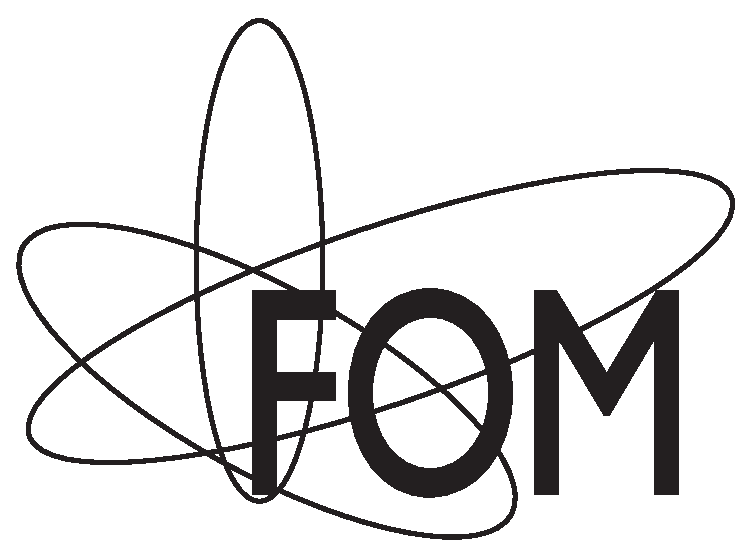
\includegraphics[height=2.5cm]{figures/FOMlogo_zw}
\hfill
\includegraphics[height=2cm]{figures/2d_NWO_LogoBasis_Zw}

\vspace{.5cm}

\noindent
This work is part of the research programme of the Foundation for
Fundamental Research on Matter (FOM), which is part of the Netherlands
Organisation for Scientific Research (NWO).  It was carried out at the
National Institute for Subatomic Physics (Nikhef).


% Actual 'titlepage'

\cleardoublepage
\thispagestyle{empty}

\begin{center}

\vspace*{2cm}

\textlarger[3]{THE HISPARC COSMIC RAY EXPERIMENT}
\\[1em]
\textlarger[1]{DATA ACQUISITION AND RECONSTRUCTION OF SHOWER~DIRECTION}


\begin{onehalfspace}

\vspace{2cm}

PROEFSCHRIFT

\vspace{2cm}

ter verkrijging van\\
de graad van doctor aan de Universiteit Twente,\\
op gezag van de rector magnificus,\\
prof. dr. H. Brinksma,\\
volgens besluit van het College voor Promoties\\
in het openbaar te verdedigen\\
op woensdag 17 oktober 2012 om 14.45 uur\\

\vspace{1cm}

door

\vspace{1cm}

David Boudewijn Reinder Alexander Fokkema\\
geboren op 14 december 1978\\
te Alphen aan den Rijn

\end{onehalfspace}
\end{center}


\newpage


\noindent
Dit proefschrift is goedgekeurd door:
\begin{tabbing}
Promotor: \hspace{2cm} \= prof. dr. ing. B. van Eijk \\
Assistent-promotor: \> dr. J. Steijger
\end{tabbing}
